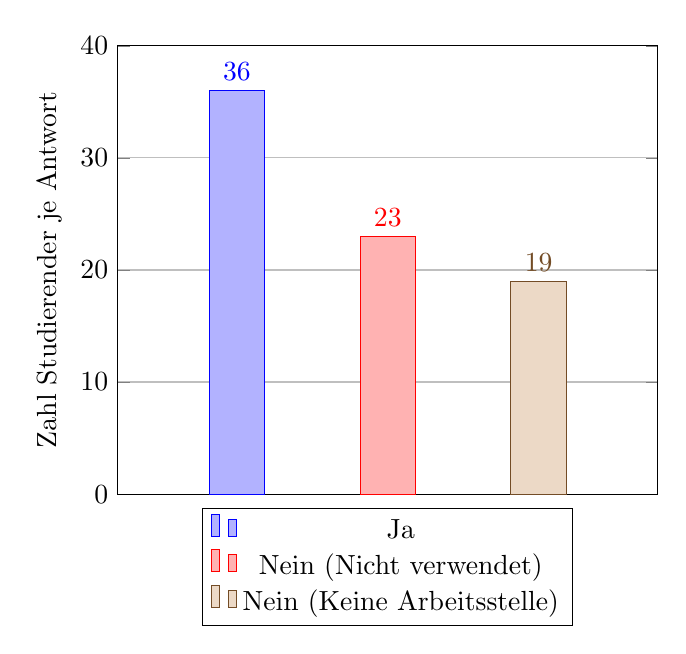
\begin{tikzpicture}
    \begin{axis}[
        x tick label style={
            /pgf/number format/1000 sep=},
        ylabel=Zahl Studierender je Antwort,
        enlarge x limits=1,
        ymax=40,
        ymin=0,
        legend style={at={(0.5,-0.03)},
        anchor=north,legend columns=1},
        ybar,
        bar width=20pt,
        xtick=\empty,
        xticklabels={},
        nodes near coords,
        grid=major
    ]
    
    \addplot coordinates {(1,36)}; % Ja
    \addplot coordinates {(2,23)}; % Nein
    \addplot coordinates {(3,19)}; % Nein (Keine Arbeit momentan)
    
    \legend{Ja, Nein (Nicht verwendet), Nein (Keine Arbeitsstelle)}
    \end{axis}
\end{tikzpicture}